\documentclass[12pt,a4paper]{article}
\usepackage[utf8]{inputenc}
\usepackage{amsmath}
\usepackage{amssymb}
\usepackage{placeins}
\usepackage{amsthm}
\usepackage{amsfonts}
\usepackage{graphicx}
\usepackage[all]{xy}
\usepackage{cite}
\usepackage{tikz}
\usepackage{verbatim}
\usepackage{float}
\usepackage{bbm} %indicator function 1 package
\usepackage{bbold} %indicator function 1 package with bold
\usepackage[left=2cm,right=2cm,top=3cm,bottom=2.5cm]{geometry}
\usepackage{hyperref}
\usepackage{caption}
\usepackage{subcaption}
\usepackage{psfrag}
\usepackage{mathrsfs}
\author{Yusuf Brima}
\title{Towards understanding Potential Evapotranspiration across 10 African cities using Statistical Machine Learning}
\begin{document}
\maketitle
\thispagestyle{empty}
\pagebreak
\begin{abstract}
The world is rapidly evolving at an unprecedented rate largely due to human actions on the environment. The effects of  this  change is being noticed through variable patterns in the climate across the global which is projected to have unforeseen consequences in the near and far future. Climate change is a prevailing threat existential crisis we are facing as a human species which if not mitigated will have devastating consequences on us and our surrendering fauna and flora. Therefore,  in this work,  we use state-of-the-art Hierarchical Cluster Analysis (CA) and Principal Component Analysis (PCA) algorithms. We found four clusters for the 10 cities with similar Potential Evapotranspiration and using PCA (both non rotated and rotated) to identify the underlying processes that gave rise to the factors of variation int the data set wherein we identified two principal components using varimax that explain nearly 90 per cent of variability in the data. 
\end{abstract}
\pagenumbering{roman}
\pagebreak
\tableofcontents
\pagebreak
\section{Introduction}
\pagenumbering{arabic}
Climate change is one of the prevailing  existential crisis we are facing as a human species which if not mitigated will have devastating consequences on us and earth's biodiversity. This effect is large since the climatic condition of the atmosphere dictates the survival ability of all life forms, the civilization we take for granted is hinged on our ability to produce food on an industrial scale to cater for the soaring global population, availability of clean air and freshwater systems as well as the ozone layer of the atmosphere to shield us from ultraviolet radiation from the sun.
A scholarly exposition of the effect of climatic changes is crucial for especially the developing world where the effect of such changes is projected to have greater impact leading to extreme events such as droughts, flooding,  hurricanes, famines, the rise of sea levels along coastal regions \cite{mitchell1989greenhouse, wang2018effect}.  These events starkly have the potential to undermine economic activities and political stability. 

Evapotranspiration (ET) is an important component of the hydrologic cycle and involves the exchange of water between the surrounding water bodies, soil, crop surfaces, and the atmosphere\cite{katul2012evapotranspiration}. Crop growth and yields are largely affected by the rate of ET, especially in semi-arid areas where the rate of ET is high and rainfall is not sufficient and reliable to add more water into the soil for crop use. Solar radiation, relative humidity, air temperature, rainfall, and wind velocity are some of the meteorological factors that affect ET.
Therefore, we take a scholarly approach to study the Potential Evapotranspiration across ten African cities to discover insights that can help inform climate change mitigation policy formulation using state-of-the-art Statistical and Machine Learning techniques.
\section{Research Problem}
Understanding the effect of evapotranspiration patterns of different geographic regions across the African continent is pivotal to coordinated climate action and policy formulation. However, this process involves aggregating big data from locations that have varied underlying factors of variation in the data generation processes.
\section{Research Objective}
\begin{enumerate}
\item[(I)] The object of this research is to explore the characteristics of three Cluster Analysis (CA) algorithms using the provided climate dataset over the ten African cities (Kamembe, Kayonza, Kigali, Koulikoro, Lagos, Lome, Maseno, Mombasa, Musanze, Nairobi ) using evapotranspiration.  
This is done to show the sensitivity of the grouping to the three Cluster Analysis algorithms (single linkage, average linkage,  and Ward’s algorithm), and make a comparative analysis the results as well as a physical interpretation of such findings.
\item[(II)] The second object of this work is to study the characteristics of Principal Component Analysis (PCA) algorithm and contrast it with CA using the evapotranspiration data set in question from ten African cities.  We seek to explore the sensitivity
of PCA analysis to (i) rotated and (ii) non-rotated PCA methods and the temporal variation of the  Principal Factors (PFs) over the study period.  We give physical interpretations of our findings in comparison with the objective I.
\item[(III)] Thirdly, we seek to explore the time series patterns in the two Principal Factor scores from PCA over the cities. The primary motive for this approach is to study the the processes that underpin the variability of Potential Evaporation across the 10 cities being studied. This will considerably help us find trends and periodicity in those scores which will further help in developing hypothesis about their physical interpretations.
\end{enumerate}
\section{Research Methodology}
\subsection{Evapotranspiration}
Potential Evapotranspiration (PET) is the sum of water evaporation and transpiration from a surface area to the atmosphere over a given time\cite{van1966potential}.  
 It only occurs at the potential rate when the water available for this process is non-limiting. The rate of evaporation depends on climatic conditions, specifically the radiative energy of the sun, wind, the vapour deficit of the air, and temperature. Potential evaporation is often calculated from these measurements using the Penman Monteith equation. Evaporation accounts for the movement of water to the air from sources such as the soil, canopy interception, and water bodies as depicted in Figure \ref{fig:evapo}.
\begin{figure}[!h]
			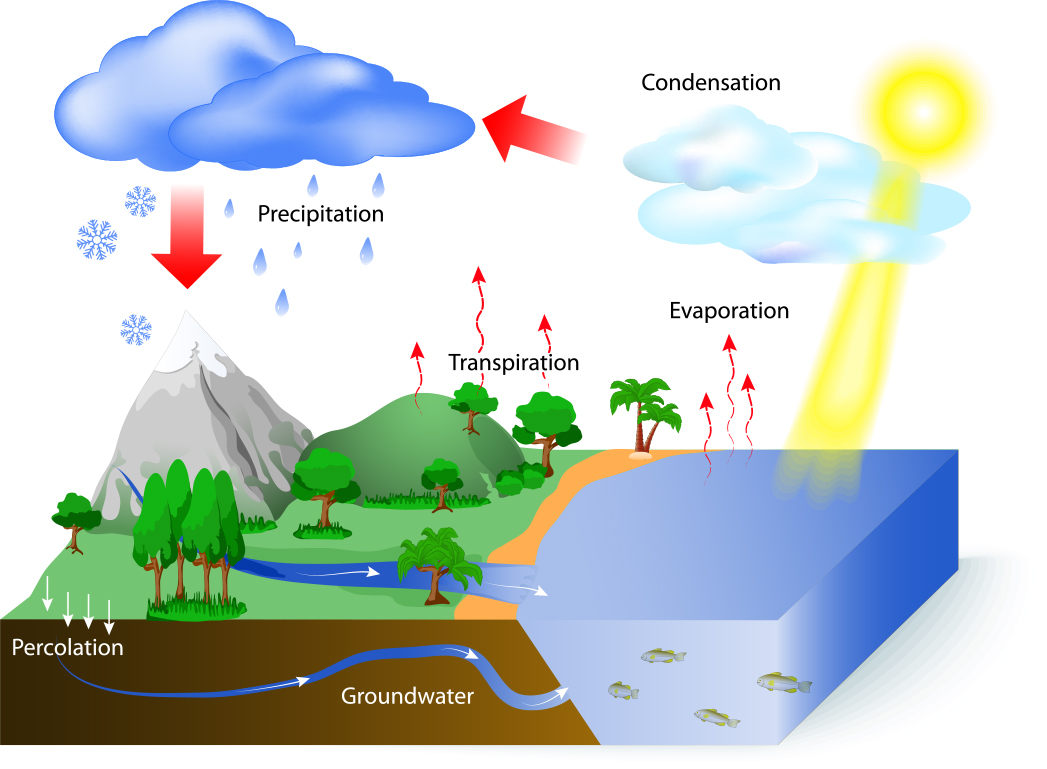
\includegraphics[width=430pt,  height=215pt]{./gaphics/evapotranspiration.jpg}
			\caption{Illustration of Evapotranspiration}
			\label{fig:evapo}
\end{figure}
\subsection{Data set}
We have utilised a secondary data source of Potential Evapotranspiration in this report from ten West and East African cities: Kamembe,  Kayonza,  Kigali,  Koulikoro,  Lagos,  Lome,  Maseno,  Mombasa,  Musanze,  Nairobi which have different geographic conditions.  This consists of 10 variables (i.e.,  evapotranspiration for each city) and 612 observations (monthly averaged evapotranspiration) from January 1960 to December 2010 (50 years).
\begin{figure}[!h]
	  \centering
        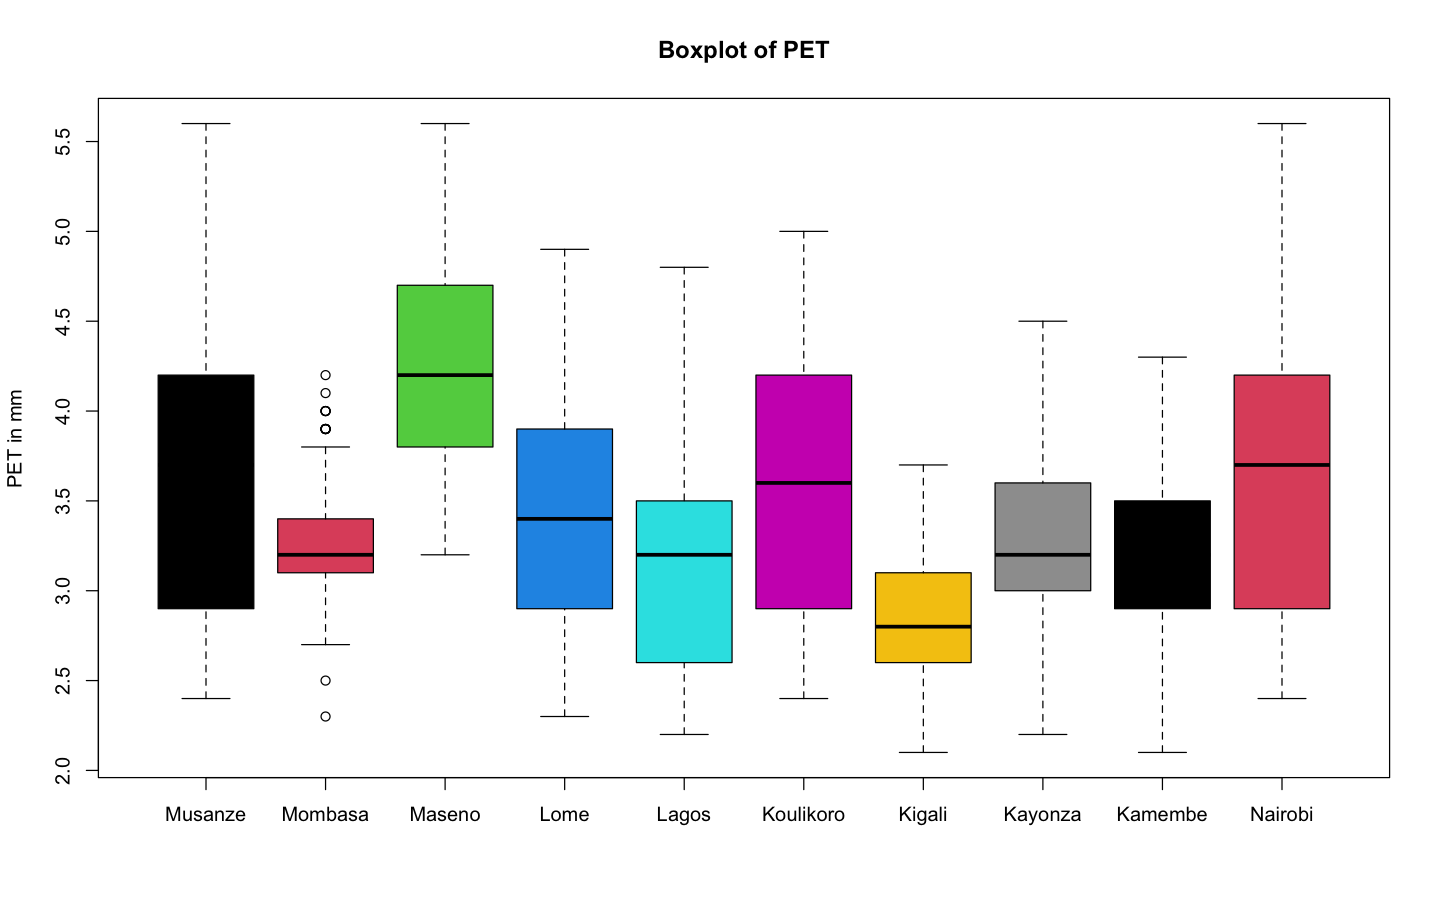
\includegraphics[height=3.2in]{./gaphics/q001_box.png}
        \caption{Summary boxplot of the dataset}
        \label{fig:box_plot}
\end{figure}

\subsection{Research Instruments}
In this research, we use Cluster Analysis technique to group the ten West and East African cities (Kamembe, Kayonza, Kigali, Koulikoro, Lagos, Lome, Maseno, Mombasa, Musanze, Nairobi) based on their evapotranspiration.
With the CA algorithm, we explored three different linkage methods: single linkage,  average linkage,  and Ward’s algorithm to investigate their effect groupings of the cities\cite{nielsen2016hierarchical}.

We further subject the same dataset to PCA algorithm with a goal of understanding the principal factors of variation that impact the evapotranspiration process for the cities in being studied with  sensitivity of PCA analysis to (i) rotated and (ii) non-rotated methods. Using the principal factors scores from PCA, we proceed with time-series analysis to further shed insight into how the variability of the processes that underlie potential evapotranspiration with respect to time.  
The primary computational tool for our experiment is the R programming language primarily because it is well suited and expressive to undertake high-level rapid exploratory data analysis for scientific reporting as well as being able to automate repetitive predictive analytic processes which all aid reproducibility of research.
\pagebreak
\section{Results and Discussions}
\subsection{Results}
In this section of report, we present the empirical observations after carrying out CA, PCA,  and time-series analysis of the Potential Evapotranspiration data set for the ten cities being studied.
\subsubsection{Cluster Analysis}
\begin{figure}[!h]
    \centering
    \begin{subfigure}[t]{0.3\textwidth}
        \centering
        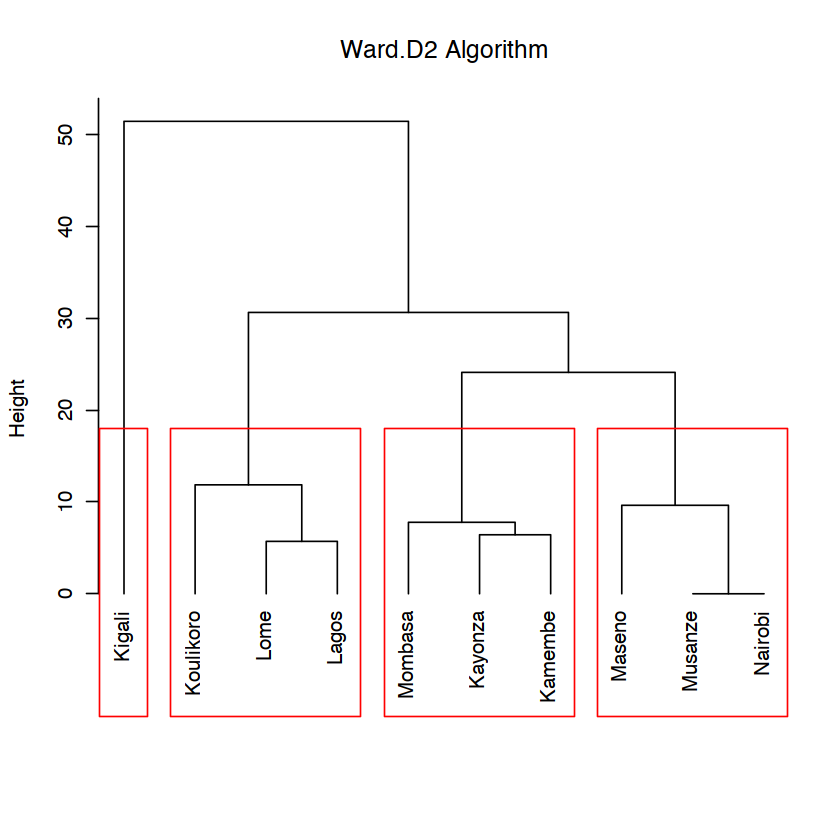
\includegraphics[height=1.8in]{./gaphics/q001_a.png}
        \caption{}
    \end{subfigure}%
    ~ 
    \begin{subfigure}[t]{0.3\textwidth}
        \centering
        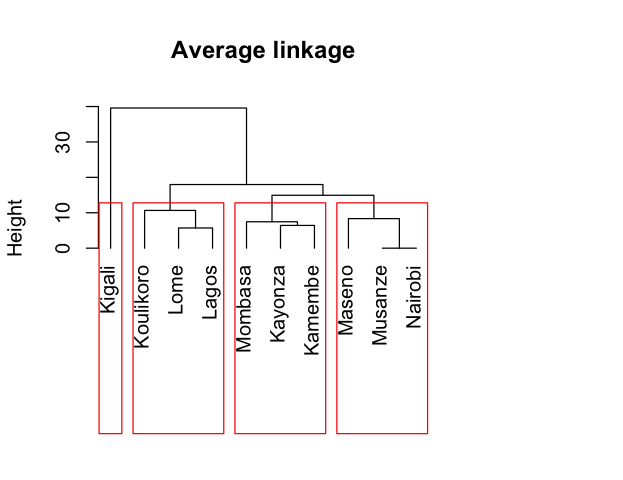
\includegraphics[height=1.8in]{./gaphics/q001_b.png}
        \caption{}
    \end{subfigure}%
    ~ 
    \begin{subfigure}[t]{0.3\textwidth}
        \centering
        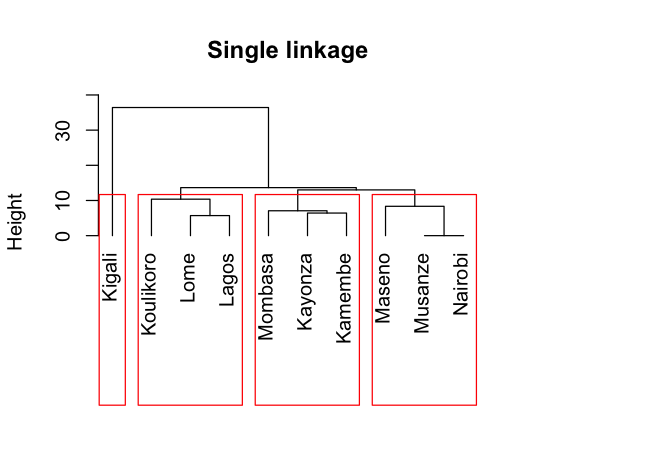
\includegraphics[height=1.8in]{./gaphics/q001_c.png}
        \caption{}
    \end{subfigure}
    \caption{Cluster Analysis with 3 distinct linkage algorithms}
     \label{fig:cluster_algorithms}
\end{figure}
The dendogram in Figure 2 presents the impact of using Ward.D2,  Average and Single linkage algorithms on the data set using a cluster value (K = 4). The red rectangles in the sub figures indicate cities that belong to the same evapotranspiration grouping thereby resulting on four clusters for the 10 cities in each on the linkage algorithms. From Figure 2 (a,b, and c), the tree linkage methods yield the same clustering results with 4 clusters each where kigali is the outlier in the dataset.
\begin{figure}[!h]
	  \centering
        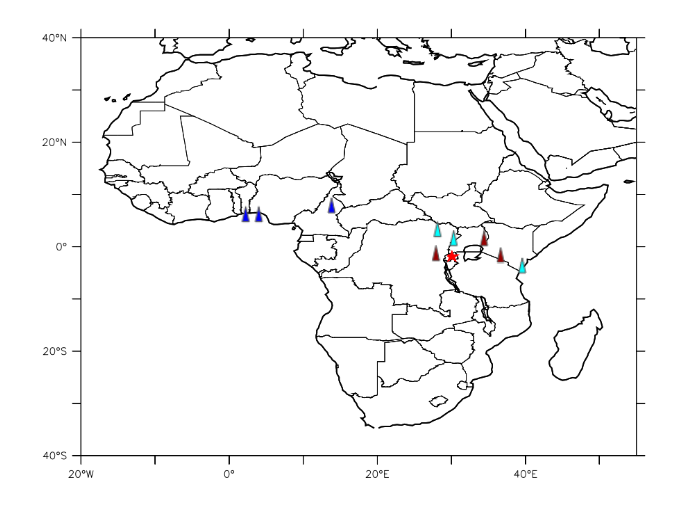
\includegraphics[height=2.4in]{./gaphics/cluster_map.png}
        \caption{Map representation of the clustered cities}
        \label{fig:cluster_map}
\end{figure}

In Figure \ref{fig:cluster_map}, we overlay the Ward.D2 cluster result onto the coordinates (longitude and latitude) of the 10 cities to infer physical and geographical interpretation of the results.  Such visual representation of the clustered data gives rise to rich geographical interpretation for the trend of Potential Evapotranspiration in the cities being studied.
One of our primary observation is, cities have been clustered based on their underlying topographic, geographic and climatic conditions. The cities on the equator generally have a tropical rain forest or equatorial climate. Distinct seasons are usually absent and in some places, however, cold currents trigger tropical monsoon climates accompanied by a dry season. The average temperature of the equatorial countries is around $30^{\circ}$C during the day\cite{webb1960thermal}.
Kigali stands out as the outlier in the city clusters with a mean PET of 2.818mm largely due to the unique topography of the Rwanda and its wide range of geographical landscapes and micro-climates. 
\subsubsection{Principal Component Analysis}
PCA is one of the popular dimensionality reduction algorithms,  it extracts fewer and independent underlying factors of variation around which the data variance is organised.  This is achieved by identifying principal processes that explain the largest variability in the data set. 
Therefore, in this study, our principal motivation for factor analysis using PCA is to understand the underlying principal processes that drive Potential Evapotranspiration across the ten cities. The Figures (a) and (b) below indicate the screeplot of the eigenvalues and the Percentage Variance Explained (PVE) of the ten principal components using varimax rotation.
Figures (a) and (b),  clearly indicate that the first and second principal components explain nearly 90 per cent of the variability in  the underlying processes that generated the data.
\begin{figure*}[!h]
    \centering
    \begin{subfigure}[t]{0.5\textwidth}
        \centering
        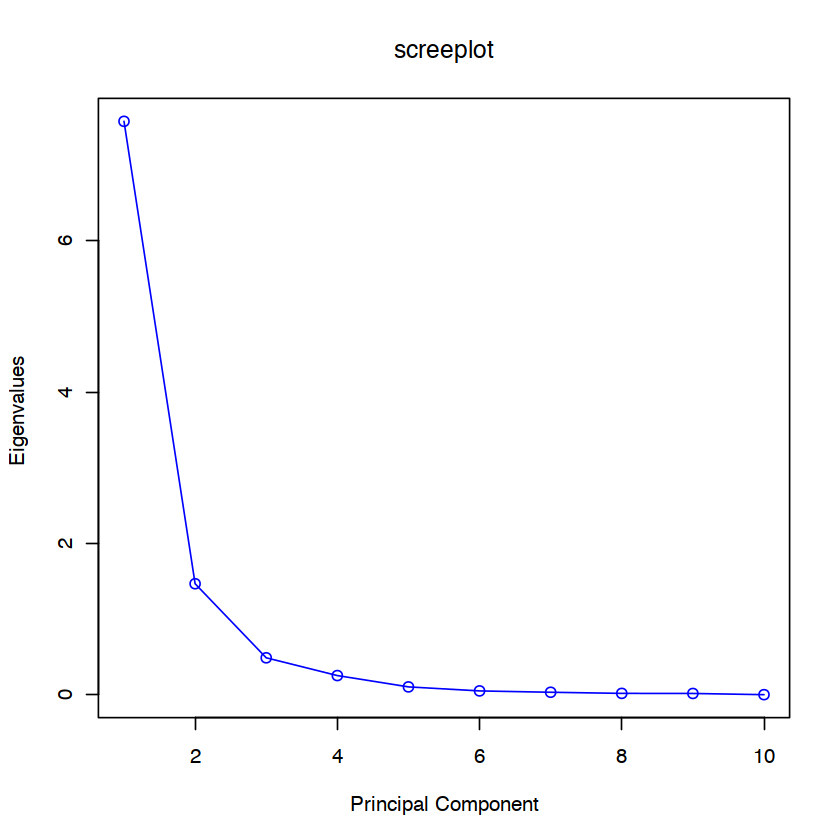
\includegraphics[width=\textwidth,height=200pt]{./gaphics/q002_b.png}
        \caption{}
    \end{subfigure}%
    ~ 
    \begin{subfigure}[t]{0.5\textwidth}
        \centering
        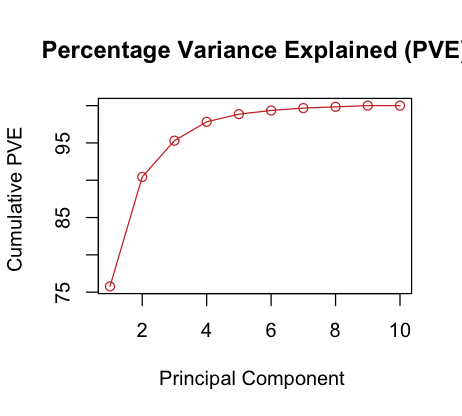
\includegraphics[width=\textwidth,height=200pt]{./gaphics/q002_c.png}
        \caption{}
    \end{subfigure}
    \caption{Principal Component Analysis}
\end{figure*}
To further understand the effect of the underlying processes of the principal components, we have plotted a 10 year window time series for the two rotations in the figure below.
\textbf{PCA Loadings (unrotated)}
\begin{verbatim}
Loadings:
          PC1    PC2    PC3    PC4    PC5    PC6    PC7    PC8    PC9    PC10  
Musanze    0.912  0.309 -0.241                                                 
Mombasa    0.899  0.211  0.348 -0.109                                          
Maseno     0.856  0.342 -0.333         0.143 -0.129                            
Lome       0.901 -0.321         0.255                                          
Lagos      0.882 -0.361         0.272                                          
Koulikoro  0.907 -0.343                0.195  0.132                            
Kigali    -0.360  0.862  0.244  0.246                                          
Kayonza    0.952  0.131  0.170 -0.153               -0.117                     
Kamembe    0.961         0.200 -0.126                       0.103              
Nairobi    0.912  0.309 -0.241                                                 

                 PC1   PC2   PC3   PC4   PC5   PC6   PC7   PC8   PC9 PC10
SS loadings    7.578 1.466 0.487 0.252 0.103 0.050 0.032 0.017 0.016    0
Proportion Var 0.758 0.147 0.049 0.025 0.010 0.005 0.003 0.002 0.002    0
Cumulative Var 0.758 0.904 0.953 0.978 0.989 0.994 0.997 0.998 1.000    1
\end{verbatim}

The from the unrotated PCA loads above, PC1 and PC2  account for 09.04 per cent of the cumulative variance in the dataset. This means, we can derive a new projection from the dataset which is high-dimensional to a two-dimensional projection that explains 90.04 per cent of the variability in the dataset. Such a method can allow us to compress, visualise and perform further analysis of the data to gain better insight.

We present the varimax (the method frequently used in scientific exploratory analysis of high-dimensional data) rotated PCA loadings below which was further used to gain deeper into into the underlying factors of variation in the data set.

\textbf{PCA Loadings (rotated)}
\begin{verbatim}
Loadings:
          RC3    RC1    RC4    RC2    RC5    RC7    RC6    RC9    RC8    RC10  
Musanze    0.866  0.400  0.272               -0.110                            
Mombasa    0.443  0.830  0.328                                                 
Maseno     0.899  0.301  0.233                0.200                            
Lome       0.378  0.397  0.750  0.352                       0.112              
Lagos      0.333  0.380  0.777  0.358                                          
Koulikoro  0.389  0.481  0.534  0.478  0.323                                   
Kigali                  -0.242 -0.970                                          
Kayonza    0.547  0.737  0.322  0.132                0.162                     
Kamembe    0.504  0.748  0.373  0.178                              0.119       
Nairobi    0.866  0.400  0.272               -0.110                            

                 RC3   RC1   RC4   RC2   RC5   RC7   RC6   RC9   RC8 RC10
SS loadings    3.463 2.736 2.061 1.479 0.121 0.066 0.034 0.022 0.018    0
Proportion Var 0.346 0.274 0.206 0.148 0.012 0.007 0.003 0.002 0.002    0
Cumulative Var 0.346 0.620 0.826 0.974 0.986 0.993 0.996 0.998 1.000    1
\end{verbatim}

\begin{figure*}[!h]
    \centering
    \begin{subfigure}[t]{0.5\textwidth}
        \centering
        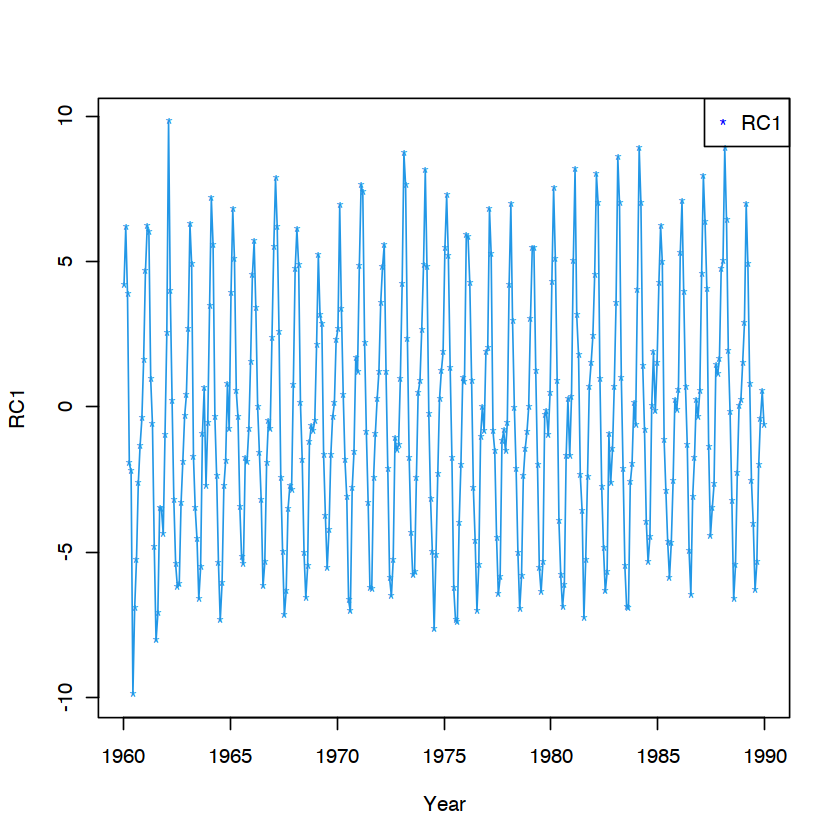
\includegraphics[width=\textwidth,height=170pt]{./gaphics/q002_e.png}
        \caption{Time series of PCA RC1} 
    \end{subfigure}%
    ~ 
    \begin{subfigure}[t]{0.5\textwidth}
        \centering
        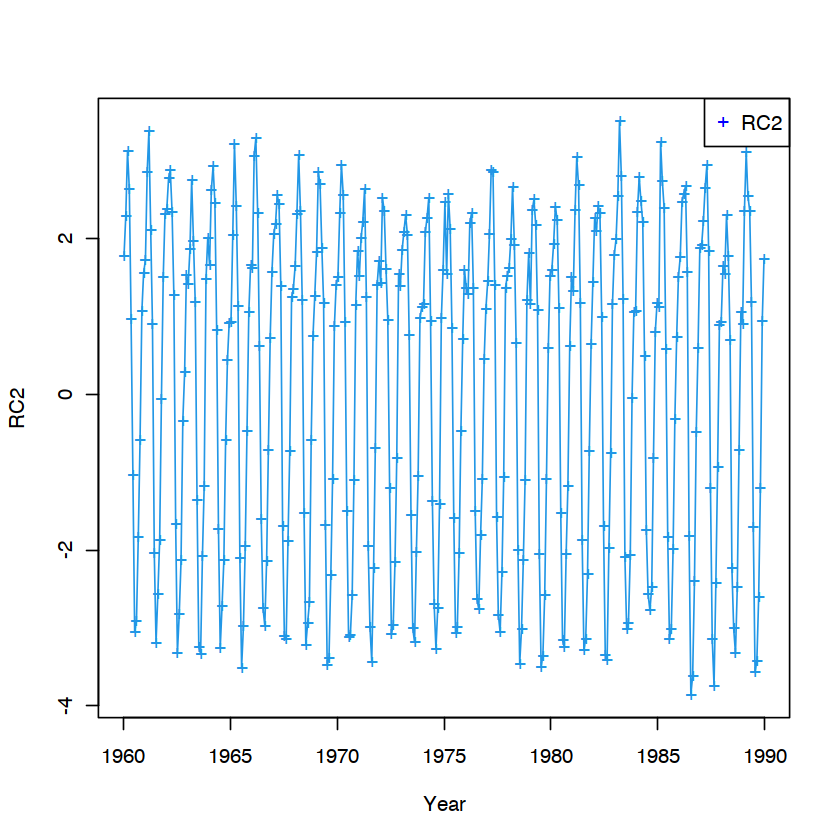
\includegraphics[width=\textwidth,height=170pt]{./gaphics/q002_e2.png}
        \caption{Time series of PCA RC2} 
    \end{subfigure}
    \caption{Principal Component Analysis: Rotations}
    \label{fig:time_series}
\end{figure*}


Figure  \ref{fig:time_series} below describes proportion of variability captured by each Principal  Rotated Components (RC1 and RC2) on the
original data and the component scores.  The scores show how each process varies in the time domain.  RC1 was most active in around 1962 through 1966 with temporal spikes in approximately in a 15 year window as shown in Figure  \ref{fig:time_series} (a). There overall trend shows that the principal component RC1 periodically have strong influence on the amount of Potential Evapotranspiration of the ten cities thereby account for 62 per cent of PET variability.

Our analysis of RC2 show a pattern akin to RC1, the process was most dominate in mid 1960s and least active around 1974 most likely due to factors that influence evapotranspiration such as solar plant's growth stage or level of maturity, percentage of soil cover, radiation, humidity, temperature, and wind.
\subsubsection{Time-series Analysis}
A time series is a series of data points indexed (or listed or graphed) in time order\cite{wei2006time}. Most commonly, a time series is a sequence taken at successive equally spaced points in time. Thus it is a sequence of discrete-time data. To deploy time series analysis the dataset must satisfy these two conditions. Time series analysis comprises of various methods that analyses time. The aim of this task was to explore the time series patterns in potential evapotranspiration PCA scores (RC1 and RC2) data and the relationships between the two variables. This is important for the purpose of learning and analysing the patterns. As a result it helps to study the past and predict the future.
\begin{figure*}[!h]
    \centering
    \begin{subfigure}[t]{0.5\textwidth}
        \centering
        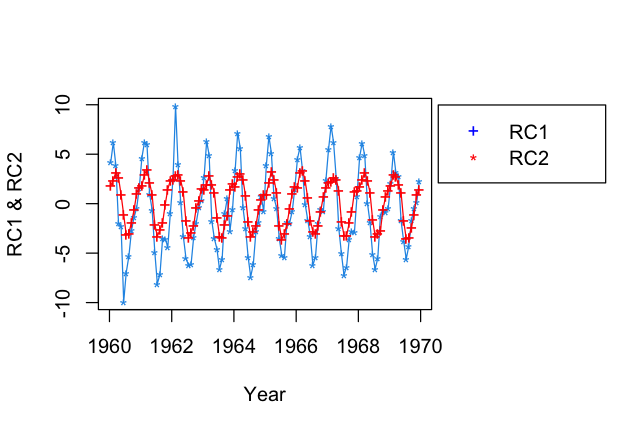
\includegraphics[width=\textwidth,height=170pt]{./gaphics/q002_d.png}
        \caption{RC1 and Linear Fit} 
    \end{subfigure}%
    ~ 
    \begin{subfigure}[t]{0.5\textwidth}
        \centering
        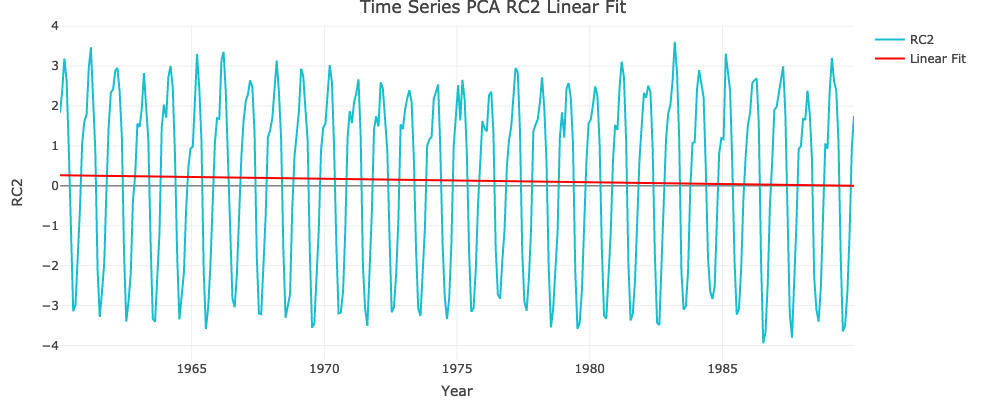
\includegraphics[width=\textwidth,height=170pt]{./gaphics/q002_f.png}
        \caption{RC2 and Linear Fit} 
    \end{subfigure}
    \caption{Time series of PCA Scores: Linear Fit}
    \label{fig:linear_fit}
\end{figure*}

We have shown a linear trend in Figure \ref{fig:linear_fit} (a) and (b) where (a) shows a slightly steady rise over the decades of the observations whilst (b) shows a steady declining trend over the same period.  This  allows us the hypothesize that  process RC1 is underpins the gradual rise in PET and process RC2 is responsible for the steady fall of PET over three decades in the 10 cities.

In a further analysis of the PCA scores, we have  used differencing to remove a trend or seasonal effects to held shed more light on the underlying factors of variability in the two processes.  This  works by removing linear and non-linear trends as well as various seasonal features that might be evident in the data.  A plot of the detrended scores is shown in Figure  \ref{fig:detrended_ts} (a) and (b) below.  
\begin{figure*}[!h]
    \centering
    \begin{subfigure}[t]{0.5\textwidth}
        \centering
        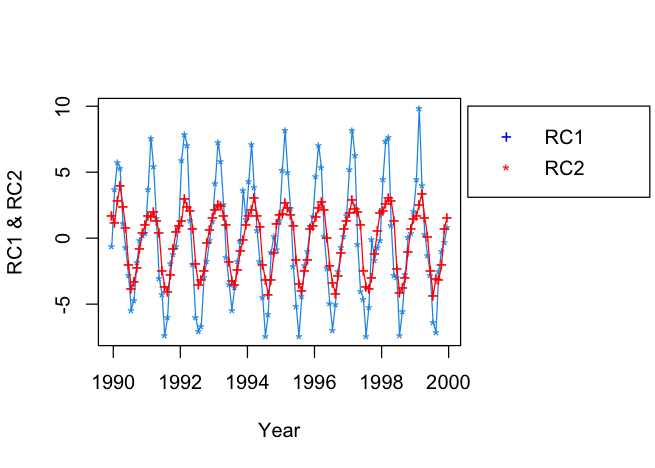
\includegraphics[width=\textwidth,height=170pt]{./gaphics/q002_g.png}
        \caption{}
    \end{subfigure}%
    ~ 
    \begin{subfigure}[t]{0.5\textwidth}
        \centering
        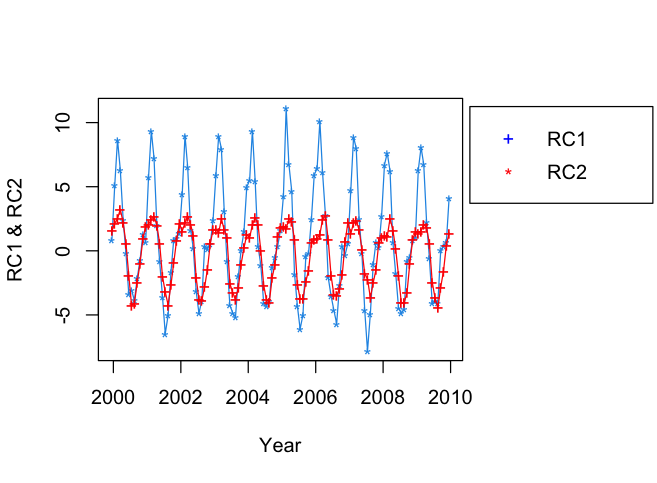
\includegraphics[width=\textwidth,height=170pt]{./gaphics/q002_h.png}
        \caption{}
    \end{subfigure}
    \caption{Principal Component Analysis: detrended}
    \label{fig:detrended_ts}
\end{figure*}

In Figure  \ref{fig:factor_corr} (a) and (b), we have show correlation matrix plots for the Rotation Components and the PET for the ten cities respectively.  Similar to the results of Cluster Analysis,  the principal rotation components for the 10 cities have correlative groupings,  e.g.,  in \ref{fig:factor_corr}  (b),  Maseno, Musanze and Nairobi have strong positive correlation which indicatively were grouped together in the hierarchical cluster analysis.
\begin{figure*}[!h]
    \centering
    \begin{subfigure}[t]{0.5\textwidth}
        \centering
        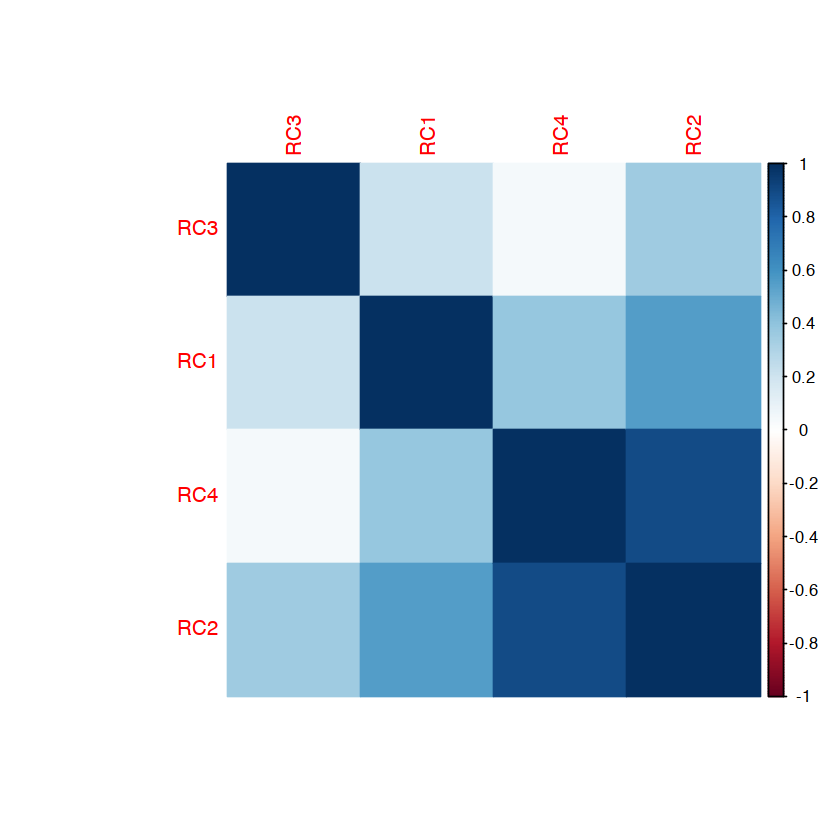
\includegraphics[height=1.9in]{./gaphics/q003_a.png}
        \caption{Rotation Components}
    \end{subfigure}%
    ~ 
    \begin{subfigure}[t]{0.5\textwidth}
        \centering
        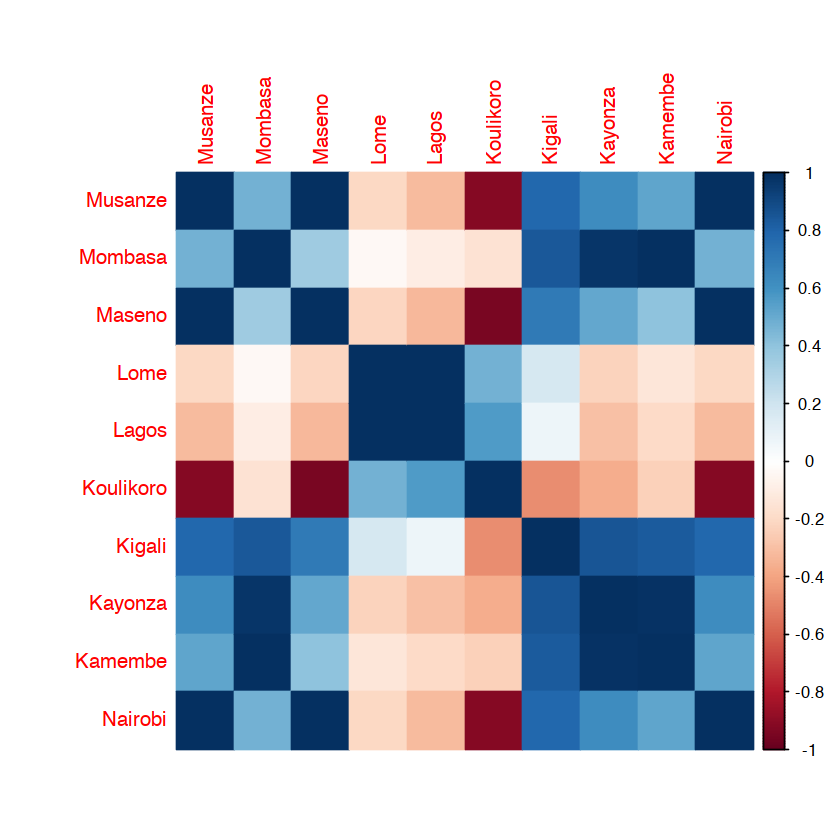
\includegraphics[height=1.9in]{./gaphics/q003_b.png}
        \caption{Cities PET}
    \end{subfigure}
    \caption{Principal Component Analysis: Factor Correlation}
    \label{fig:factor_corr}
\end{figure*}

To help use get a deeper and fine-grained understanding of the temporal variation of PET annually, we has show the plot of the potential evapotranspiration pattern yearly from 1960 through 1990 in Figure \ref{fig:periodicity} (a) and (b) for RC1 and RC2 respectively. From the plots,  we notice the that the processes that gave rise to PET are predominantly active in February to April each year peaking in March.  The second,  interesting observation is to PCA rotation component scores show a dip between June to September each year reaching the lowest point in July.  One can therefore,  theorize that, both processes follow the bi-seasonal trend of countries along the tropical and temperate belts where rainy and dry seasons are the key climatic variations.
\begin{figure*}[!h]
    \centering
    \begin{subfigure}[t]{0.5\textwidth}
        \centering
        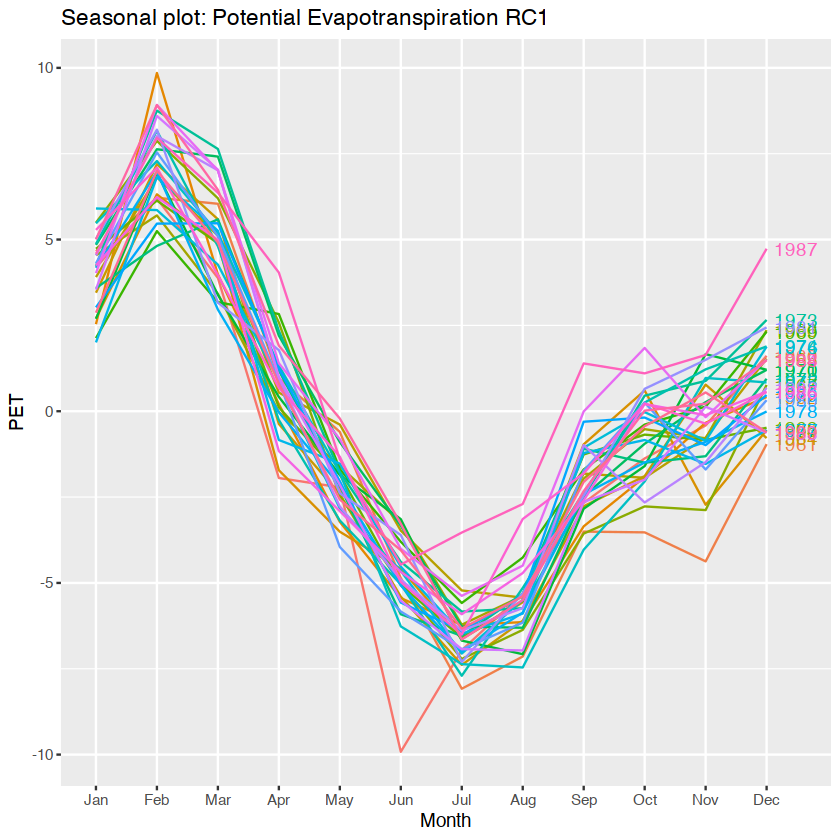
\includegraphics[width=\textwidth,height=170pt]{./gaphics/q003_d.png}
        \caption{}
    \end{subfigure}%
    ~ 
    \begin{subfigure}[t]{0.5\textwidth}
        \centering
        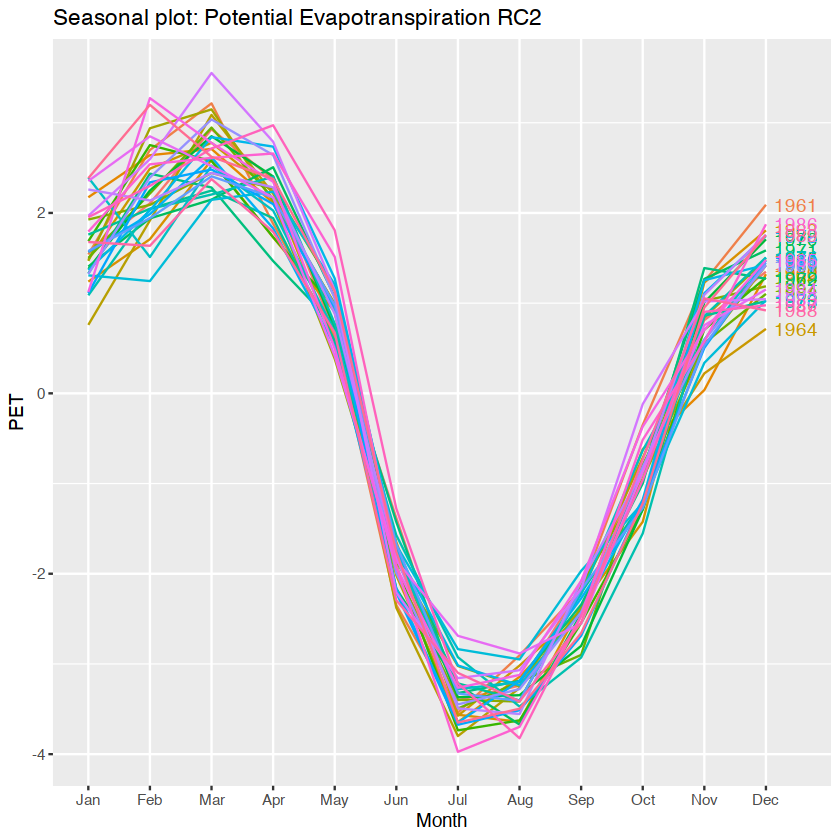
\includegraphics[width=\textwidth,height=170pt]{./gaphics/q003_e.png}
        \caption{}
    \end{subfigure}
    \caption{Principal Component Analysis: Scores Periodicity}
    \label{fig:periodicity}
\end{figure*}

%\begin{figure*}[!h]
%    \centering
%    \begin{subfigure}[t]{0.5\textwidth}
%        \centering
%        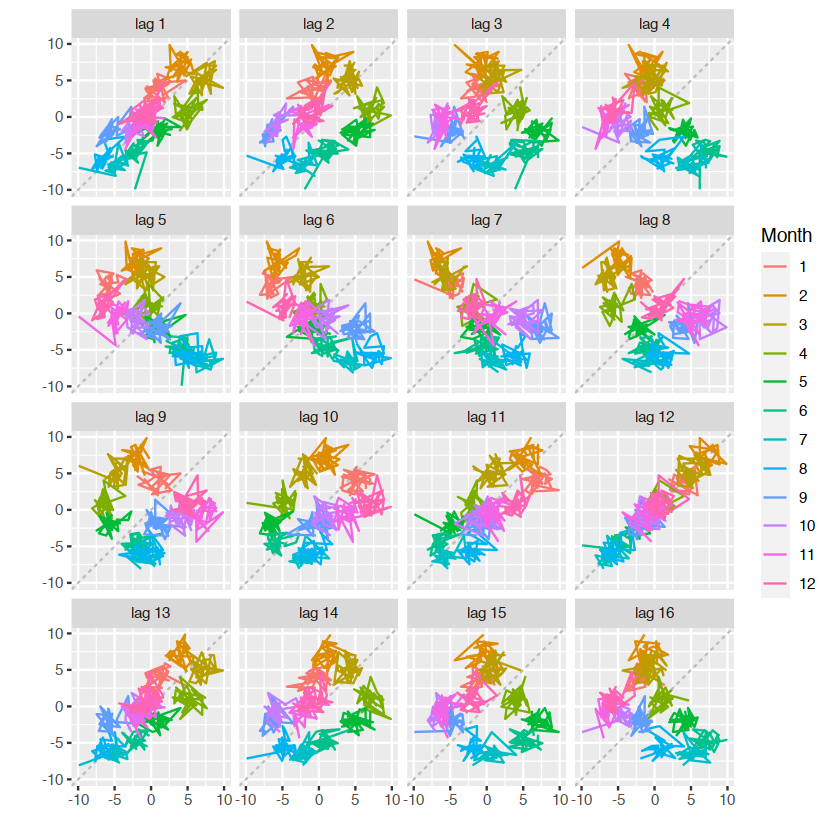
\includegraphics[width=\textwidth,height=170pt]{./gaphics/q003_f.png}
%        \caption{}
%    \end{subfigure}%
%    ~ 
%    \begin{subfigure}[t]{0.5\textwidth}
%        \centering
%        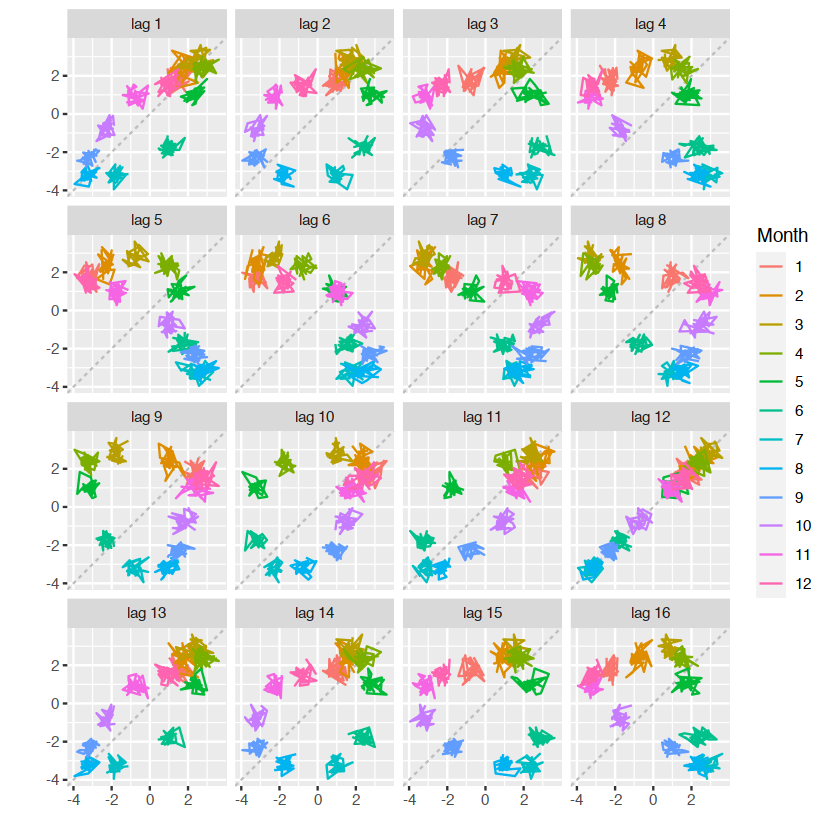
\includegraphics[width=\textwidth,height=170pt]{./gaphics/q003_g.png}
%        \caption{}
%    \end{subfigure}
%    \caption{Principal Component Analysis: Lagged Plots}
%\end{figure*}
Auto-correlation refers to the degree of correlation between the values of the same variables across different observations in the data.  The concept of auto-correlation is most often discussed in the context of time series data in which observations occur at different points in time (e.g., air temperature measured on different days of the month). 
The only significant auto-correlation at the 5\% level of significance is at lag zero. 
\begin{figure*}[!h]
    \centering
    \begin{subfigure}[t]{0.5\textwidth}
        \centering
        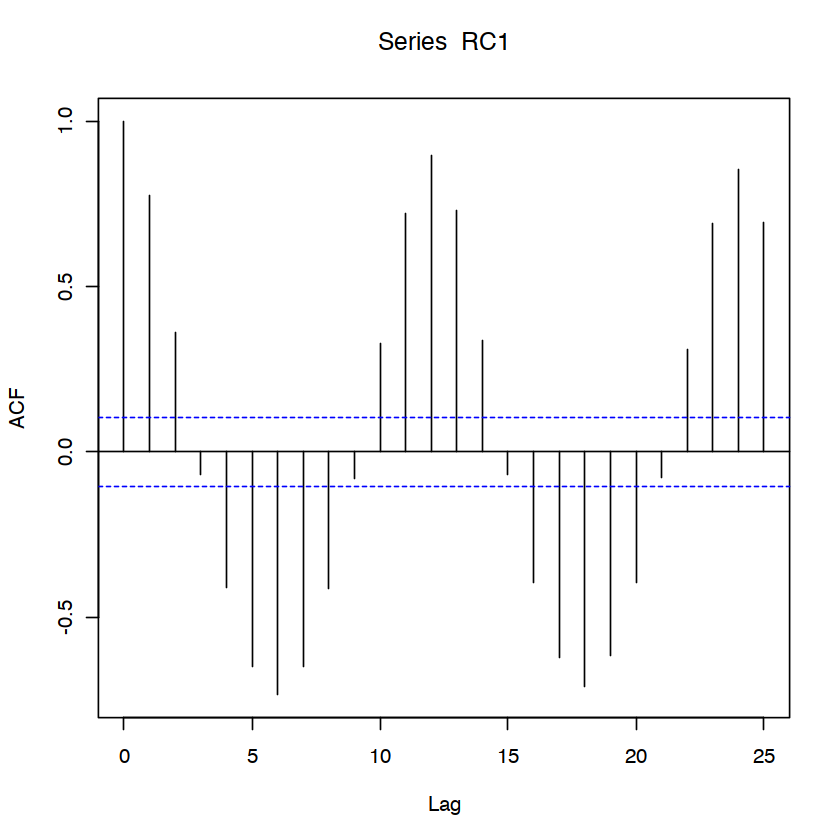
\includegraphics[width=\textwidth,height=170pt]{./gaphics/q003_h.png}
        \caption{}
    \end{subfigure}%
    ~ 
    \begin{subfigure}[t]{0.5\textwidth}
        \centering
        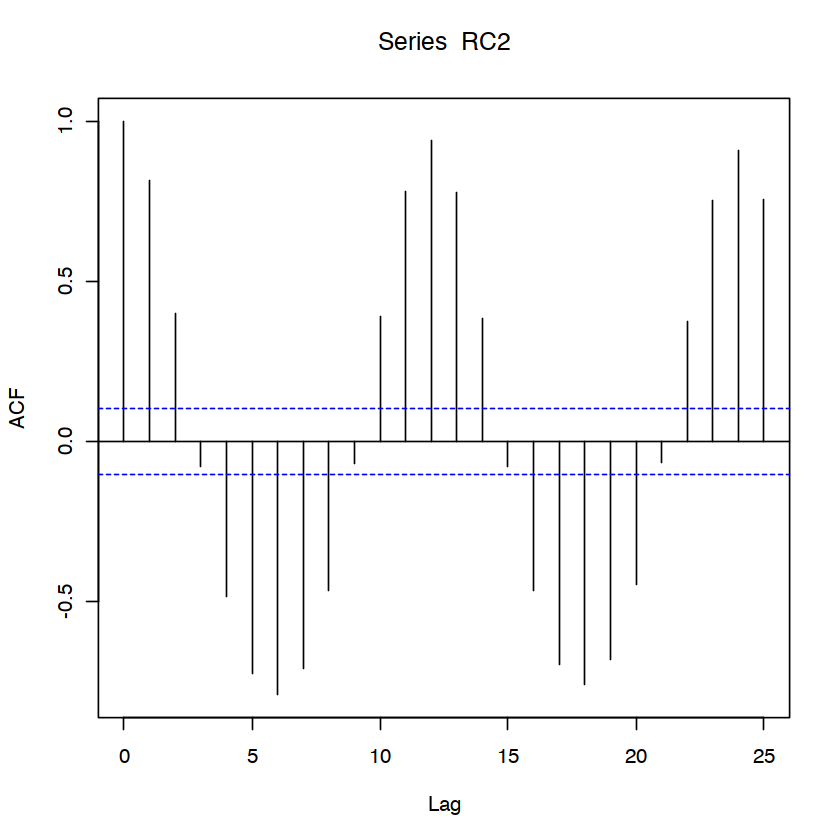
\includegraphics[width=\textwidth,height=170pt]{./gaphics/q003_i.png}
        \caption{}
    \end{subfigure}
    \caption{Principal Component Analysis: Auto-Correlation}
\end{figure*}

The sample cross correlation function (CCF) is helpful for identifying lags of one variable that might be useful predictor of another. From Figure \ref{fig:ccor},  we observe that the plot is sinusoidal and the correlation is nearly symmetrically equal.
\begin{figure}[!h]
                 \centering
                 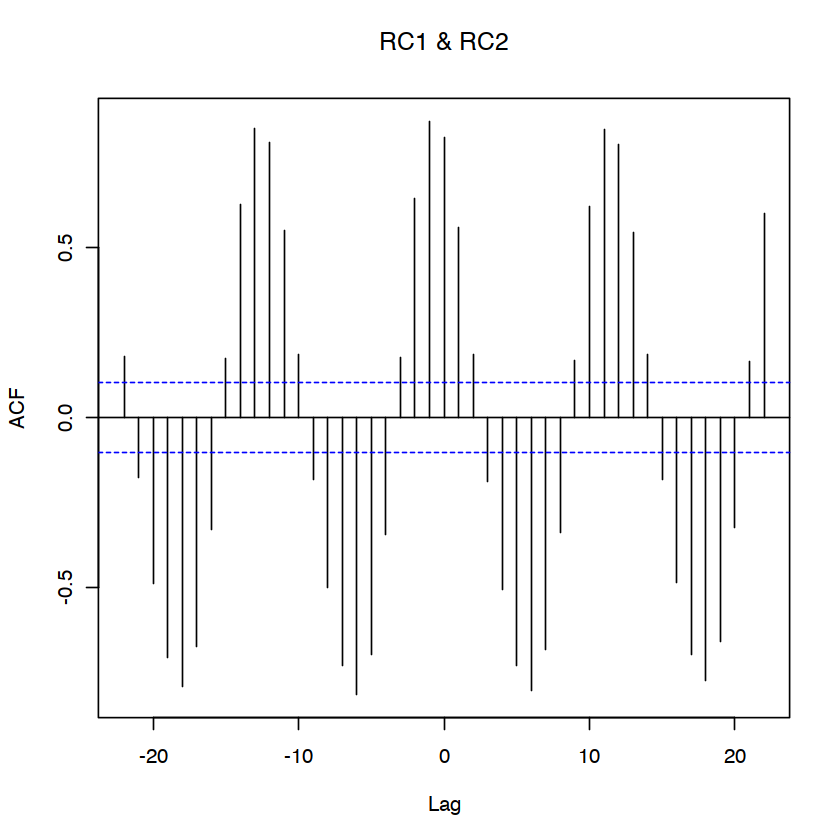
\includegraphics[width=0.98\textwidth,height=180pt]{./gaphics/q003_c.png}
\caption{Time series of PCA Rotations: Cross-correlation} 
\label{fig:ccor}
\label{fig2}
\end{figure}


\pagebreak
\section{Conclusion}
In this report,  we have explored Potential Evapotranspiration phenomenon across ten geographically different African cities using CA algorithms (using 3 distinct linkage methods) find their PET groupings, and we further,  used PCA to perform dimensionality reduction to identity the underlying processes that generated the data set \cite{wold1987principal}.    
Using CA,  we identified four distinct PET clusters as shown in  Figure 2(a).

\pagebreak
\addcontentsline{toc}{section}{References}
\bibliographystyle{ieeetr}
\bibliography{brima_yusuf_RMCS_001}
\end{document}